\chapter{理論}
\section{AIを用いた楽曲作成}
<<<<<<< HEAD
\subsection{MIDI}
MIDIとオーディオデータの形式について述べる
パソコンで用いる音楽データには大きく分けて二つある.一つ目はオーディオデータといい波形の情報を記録する形式である.二つ目がMIDIである
AIによる曲制作では主にMIDIファイルの音楽データを使用する.MIDIファイルには実際の音ではなく音楽の演奏情報(音の高さや長さなど)である.
本研究で用いるAIはこのMIDIファイルの情報を元に学習をする.また入出力の際もこの規格を用いる.
=======
%AIを用いた楽曲サービスについて述べてその中でなぜMagendaを選ぶのかを述べる
>>>>>>> 69fbd3046e62da0fe06affb2bc15d892cf1d4e2b
\subsection{Magenta}
本研究で使用するMagenta[1]は音楽などをTensorFlowを使って機械学習するライブラリであり,Google BrainがGitHab上に公開されているOSSである.
Magentaではまず学習させたい音楽のMIDIデータをNoteSequence(magentaが扱うファイル形式)とよばれるデータフォーマットに変更する.それを学習用データセットと評価用データセットに変換したあと学習を行う.
このとき,一度に学習させるデータの数,学習を行う回数,ノード数を設定する.これをパッケージ化し,MIDIファイルとして新たに楽曲を生成するという流れである.これを図2.1に示す.
\newpage
\begin{figure}[h]
\begin{screen}
\begin{center}
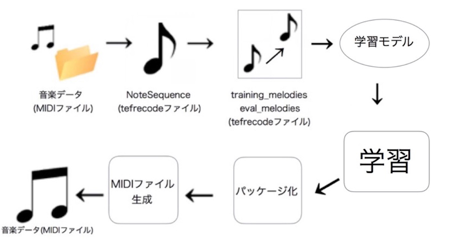
\includegraphics[scale=1.7, clip]{./img/magenta_usestep.png}
\caption{magentaによるMIDI音楽データ生成までのプロセス}
\label{fig:magentaによるMIDI音楽データ生成までのプロセス}
\end{center}
\end{screen}
\end{figure}\\
\subsection{MIDI}
%MIDIとオーディオデータの形式について述べる
パソコンで用いる音楽データには大きく分けて二つある.一つ目はオーディオデータといい波形の情報を記録する形式である.二つ目がMIDIである
AIによる曲制作では主にMIDIファイルの音楽データを使用する.MIDIファイルには実際の音ではなく音楽の演奏情報(音の高さや長さなど)である.
本研究で用いるAIはこのMIDIファイルの情報を元に学習をする.また入出力の際もこの規格を用いる.
\section{機械学習に適した開発環境について}
\subsection{CUDA}
CUDAというのは、NVIDIAが開発しているGPU上でプログラミングをするためのソフトウェアプラットフォームになります。含まれるものとしては、CUDAを実行形式に変えるコンパイラみたいなもの、それをサポートするSDK、ライブラリ、あとはデバッグツール群ですね。――CUDAを導入することによって、何がどう変わるのでしょうか?橋本:一般的に行われるプログラミングというのは、いわゆる順次処理に適したものです。それを並列化していくなかで、単に複数のプロセッサで動かせばいいということではなく、いかに無駄なく並列化するのか、というのが重要なのですが、これが非常に難しい問題なんですね。特にNVIDIAのGPUには非常に多くのプロセッシングユニットが含まれています。そしてCUDAにはこれを無駄なく活用するためのいろいろなテクニックが組み込まれています。
CUDAのプログラムを実行するにあたって、GPUはグループ化されているんですね。GPUにはたくさんのコアがありますが、プログラムは1個1個のコアを認識するのではなくて、ある一定の数でグループ化されていて、その各々のグループに対してセットのオペレーションを振り分けていくんです。これはどういうことかと言うと、コンピュータを実行するためには計算だけではなく、メモリのリードライトが必要です。実はこのメモリのリードライトってものすごく時間かかるわけですよ。だからプログラムをコアで実行しようとすると、最初にやるのはメモリリードなんです。まず、データが来るまでにすごく待ちます。計算をしたら次のデータがほしいので、また待たないといけません。すると時間軸上でプロセッサが動いてるのはココとココ(下記の画像の、上側のオレンジの部分)だけになるんです。GPUではテクスチャ処理などを実行するときに、ピクセルを順次に計算していくのですが、次のピクセルで読まなきゃいけないデータはある程度予測できるんです。必要なデータに事前にメモリーリクエストを出すんですよ。いわゆるスケジュールドアクセスですね。同じようなテクニックを使ってCUDAでも次の処理に必要なデータを先読みしようと。そうすることによって、計算処理があって、これを10スレッド走らせるときに、クロックを少しずつずらして実行していくんですね。そうするとプロセッサが無駄なく回るわけですよ。こういった処理をより書きやすくしたのがCUDAというわけです。ちなみに、CUDAの形式で書けばなんでも速くなるかというと、そうではありません。各人は事前に、どこにどういうデータがあって、どういう風に割り当てて、どういう風にアクセスさせていくかということを設計しなければダメですね。CUDAの場合は設計が一番重要になってきます。
\newpage
\subsection{開発環境}
前提としてディープラーニング(深層学習)などの用途でNVIDIA社製GPUボードを利用する場合、 ディープラーニング用フレームワーク等のソフトウェアを導入する前に 下記のNVIDIA社製ソフトウェアを導入する必要があります.
\begin{enumerate}
\renewcommand{\labelenumi}{(\arabic{enumi})}
\item CUDA Toolkit
\item PUボード用ドライバーソフトウェア
\item 追加のライブラリ(cuDNNなど
    \end{enumerate}
    Magendaプロジェクトが推奨している開発環境の構築には二つ方法があり,一つはDockerというコンテナ型の仮想化環境を構築できるオープンソースソフトウェアを用いる方法と,ローカル環境にPythonのパッケージ管理システムであるpipを用いて構築する方法の2つがある.\\
    Dockerを用いることで仮想化環境をクラウド上で共有できるサービスをであるDockerHubを使用できるため,パッケージのインストールをおこなわずにコマンド一つで環境を構築できる.
    しかし,コンテナにGPUを割り当てることは現状ではNVIDIAが公開しているOSSのnbidia-dockerという
    \begin{figure}[h]
    \begin{screen}
    \begin{center}
    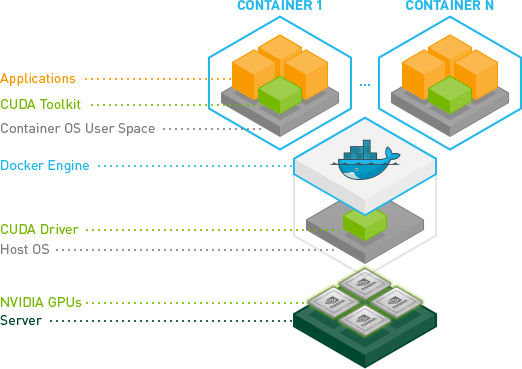
\includegraphics[scale=0.55, clip]{./img/NVIDEA_Docker.png}
    \caption{Docker用NVIDAコンテナランタイム\newline(引用:https://github.com/NVIDIA/nvidia-docker)}
        \label{img:Docker用NVIDAコンテナランタイム}
        \end{center}
        \end{screen}
        \end{figure}\\
        \newpage
        本システムの開発環境を表\ref{tab:開発環境}に示す.
        \begin{table}[h]
        \begin{center}
        \caption{開発環境}
        \label{tab:開発環境}
        \begin{tabular}{|c|p{15zw}|}
        \hline
        OS & OS X Yosemite\\
        \hline
        CPU & Intel Core i5\\
        \hline
        メモリ & 8GB\\
        \hline
        GPU & GeForce GTX 1060\\
        \hline
        使用ライブラリ & TensorFlow ,magenta\\
        \hline
        \end{tabular}
        \end{center}
        \end{table}\\
        本システムは Macbook Pro を使用しOSは OS X Yosemite を使用した.
使用するライブラリとして,ニューラルネットワークを構築できるTensorflowを利用した.